\documentclass[twoside,11pt]{article}

% Any additional packages needed should be included after jmlr2e.
% Note that jmlr2e.sty includes epsfig, amssymb, natbib and graphicx,
% and defines many common macros, such as 'proof' and 'example'.
%
% It also sets the bibliographystyle to plainnat; for more information on
% natbib citation styles, see the natbib documentation, a copy of which
% is archived at http://www.jmlr.org/format/natbib.pdf

%%%%%%%%%%%%%%%%%%%%%%%%%%%%%%%%%%%%%%%%%%%%%%%%
% Style file settings DO NOT MODIFY THIS SECTION
%%%%%%%%%%%%%%%%%%%%%%%%%%%%%%%%%%%%%%%%%%%%%%%%
\usepackage{jmlr2e}
\setlength{\parskip}{0.25em}
\renewcommand{\arraystretch}{1.2}

%%%%%%%%%%%%%%%%%%%%%%%%%%%%%%%%%%%%%%%%%%%%%%%%
% Handy packages
%%%%%%%%%%%%%%%%%%%%%%%%%%%%%%%%%%%%%%%%%%%%%%%%
\usepackage[normalem]{ulem}
\usepackage{amsmath}
\usepackage{amssymb, mathtools, amsfonts}
\usepackage{tikz}
\usepackage{tikz-qtree}
\usetikzlibrary{trees}
\usepackage{algorithm}
\usepackage[noend]{algpseudocode}
\usetikzlibrary{automata,positioning}
\usepackage{multirow}
\usepackage{hyperref}
\allowdisplaybreaks

%%%%%%%%%%%%%%%%%%%%%%%%%%%%%%%%%%%%%%%%%%%%%%%%
% Definitions of handy macros can go here
%%%%%%%%%%%%%%%%%%%%%%%%%%%%%%%%%%%%%%%%%%%%%%%%

% Operators for drawing in-text edges for PAGs, DAGs, ADMGs, CGs etc
\DeclareMathOperator{\circlearrow}{\hbox{$\circ$}\kern-1.5pt\hbox{$\rightarrow$}}
\DeclareMathOperator{\circlecircle}{\hbox{$\circ$}\kern-1.2pt\hbox{$--$}\kern-1.5pt\hbox{$\circ$}}
\DeclareMathOperator{\diedgeright}{\textcolor{blue}{\boldsymbol{\rightarrow}}}
\DeclareMathOperator{\diedgeleft}{\textcolor{blue}{\boldsymbol{\leftarrow}}}
\DeclareMathOperator{\biedge}{\textcolor{red}{\boldsymbol{\leftrightarrow}}}
\DeclareMathOperator{\udedge}{\textcolor{brown}{\boldsymbol{\textendash}}}

% Operators for relations in graphs
\DeclareMathOperator{\an}{an}
\DeclareMathOperator{\pa}{pa}
\DeclareMathOperator{\ch}{ch}
\DeclareMathOperator{\pre}{pre}
\DeclareMathOperator{\de}{de}
\DeclareMathOperator{\nd}{nd}
\DeclareMathOperator{\sib}{sib}
\DeclareMathOperator{\dis}{dis}
\DeclareMathOperator{\mb}{mb}

% Operator for ``do''
\DeclareMathOperator{\doo}{do}

% Operator for odds ratio
\DeclareMathOperator{\odds}{\text{OR}}

% Operators for optimization problems
\DeclareMathOperator*{\argmax}{arg\,max}
\DeclareMathOperator*{\argmin}{arg\,min}

% Operators for independence, expectation and calligraphy G
\def\ci{\perp\!\!\!\perp}
\newcommand{\E}{\mathbb{E}}
\newcommand{\G}{\mathcal{G}}


%%%%%%%%%%%%%%%%%%%%%%%%%%%%%%%%%%%%%%%%%%%%%%%%%%%%%%%%%%%%%%%%%%
% Pick and abbreviated title for your project and put down your
% last name. This title and your name will appear alternating
% pages of the project writeup at the top
%%%%%%%%%%%%%%%%%%%%%%%%%%%%%%%%%%%%%%%%%%%%%%%%%%%%%%%%%%%%%%%%%%
\ShortHeadings{An Abbreviated Title For Your Project If Needed}{Put your last name here}
\firstpageno{1}

\begin{document}

%%%%%%%%%%%%%%%%%%%%%%%%%%%%%%%%%%%%%%%%%%%%%%%%%%%%%%%%%%%%%%%%%%
% Insert the title of your project and details abouy you here
%%%%%%%%%%%%%%%%%%%%%%%%%%%%%%%%%%%%%%%%%%%%%%%%%%%%%%%%%%%%%%%%%%
\title{Inverting Film Negatives Using Multi-Layer Perceptrons
}

\author{\name {Kurt Gu}
		\email {kg10@williams.edu} \\
       	\addr {Computer Science \& Philosophy}
	}


\maketitle

%%%%%%%%%%%%%%%%%%%%%%%%
% Introduction
%%%%%%%%%%%%%%%%%%%%%%%%
\section{Introduction}
\label{sec:intro}
Film photography is seeing a resurgence in popularity in recent years. Users are taking analog pictures 
but what they share/publish are the digital versions of these pictures. However, existing mainstream hardware for digitizing 
film, such as scanners made by Epson, Noritsu, Fujifilm, and Imacon, have not been updated in decades, and are prohibitively expensive 
(a Nikon 9000ED scanner made 20 years ago now can sell for \$3000, and does not even support Windows 7).
The emergent alternative to digitizing film using scanners, is to use digital cameras in combination with a macro lens to take pictures 
of film directly. The advantages of this approach are clear: the hardware is more affordable, and digitizing a frame takes one second instead of 
several minutes with a scanner. However, since common print film (also known as color negative film) presents each frame in negative colors when developed, 
this approach has the inherent complication where users are required to invert their scans manually, which is time consuming and often inaccurate or inconsistent.
This project explores a machine learning approach to automate the color film inversion problem, by training a neural network to learn the mapping of colors between 
the original negative and the inverted final prints.

%%%%%%%%%%%%%%%%%%%%%%%%
% Preliminaries
%%%%%%%%%%%%%%%%%%%%%%%%
\section{Preliminaries}
\label{sec:prelims}
This project builds its model using a multi-layer perceptron (MLP), also known as a neural network, to learn the mapping function between 
the film negative and the inverted print. An MLP, somewhat obviously, is made of layers of perceptrons, 
each of which is a linear regression predictor of all the perceptron nodes in the previous layer.(See figure 1)\\
\begin{figure}
	\centering
	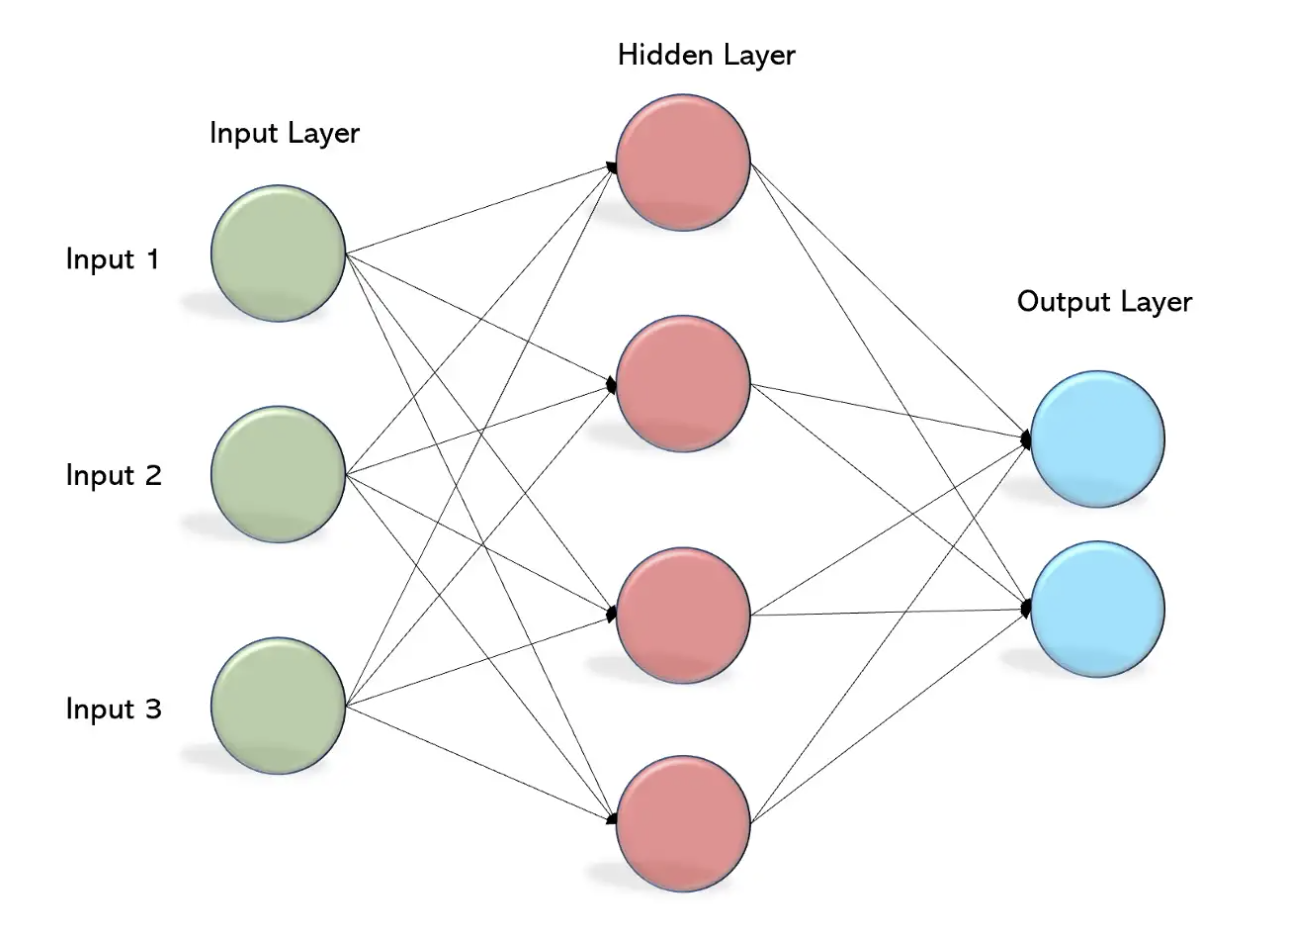
\includegraphics[width=0.5\linewidth]{mlp.png}
	\caption{MLP, or multilayer perceptron}
	\label{fig:MLP}
\end{figure}

Therefore to understand how MLPs learn, we first need to understand linear regression.\\
Linear regression produces predictions for an outcome variable $Y$ as a linear combination of learned parameters $\theta$ and input features $X$. That is, for a given example, we have the following equation that determines how we obtain a prediction $\widehat{y}$ as a function of inputs $x_1, \dots, x_d$,
	\begin{align*}
		\widehat{y} = \theta_1 x_1 + \theta_2 x_2 + \dots + \theta_3 x_d.
	\end{align*}	
	The parameters $\theta$ can be learned by minimizing a suitable loss function $L$ using gradient descent. I  use the mean squared error, which is defined for $n$ samples of data as follows: $L(\theta) \equiv \frac{1}{n} \sum_{i=1}^{n}(y_i - \widehat{y}_i)^2$. To avoid overfitting, it is common to apply a regularization penalty in conjunction with the loss: I use the L2 penalty. So, the overall function being minimized is then $L(\theta) + \lambda \sum_{j=1}^d \theta_d^2$, where $\lambda$ is a hyperparameter that will be tuned using a validation set.

An MLP is simply a combination of layers of such linear models, which add up to produce a non-linear model. 
From domain knowledge in film photography, we know that the mapping is also non-linear between film negatives and the print paper for which they were originally designed.
This indicates that it is reasonable to apply an MLP model to this problem.

%%%%%%%%%%%%%%%%%%%%%%%%
% Methods
%%%%%%%%%%%%%%%%%%%%%%%%
\section{Data}
\label{sec:data}
For this project, I'm creating my own dataset using my personal archive of film negatives taken over the years.
The input matrix is the matrix of RGB values in each of the film negative scans. The outcome matrix is intended to be an RGB value matrix 
of scans of prints made using the aforementioned negatives. However, the supplies needed to create the outcome dataset was delayed in shipping, 
so for this draft I'm instead using inversions created manually in photoshop as a temporary substitute. The one advantage to this approach is that there exists a 
pixel-to-pixel corespondence of values between my input and output. The downside and potential issue is that instead of learning a stable mapping function that exists 
in the photographic paper, the model is instead learning my film inversion technique, and I, being human, am notoriously inconsistent! So for this draft dataset I tried to only apply minimal 
and relatively consistent color-grading to the outcome images.\\

In the project repository \href{https://github.com/kg9903/CS374Project}{[link here]}  you will find a folder named "Dataset", with two folders inside labeled "Original\_resized" and "Inverted\_resized". 
Each original image, as it was scanned and cropped, is inconsistent in dimensions and each had a resolution of between 24 to 90 megapixels. 
A workstation might be able to handle these high-resolution images but not my laptop. So I've downsized all images to 256x256 pixels, 
and renamed them for easier indexing. I plan to make and add the actual paper scans in the upcoming week, likely in a higher resolution.

\begin{figure}
	\centering
	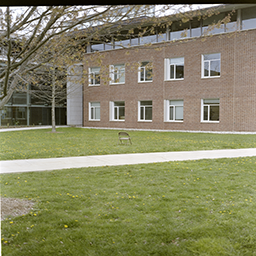
\includegraphics[width=0.6\linewidth]{validate_inverted.png}
	\caption{An inverted sample from a dataset}
	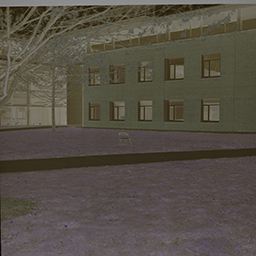
\includegraphics[width=0.6\linewidth]{validate.png}
	\caption{The original camera scan of the same image}
	\label{fig:dataset}
\end{figure}


%%%%%%%%%%%%%%%%%%%%%%%%
% Methods
%%%%%%%%%%%%%%%%%%%%%%%%
\section{Training And Validation Of Models}
\label{sec:methods}
As of right now, I trained an MLP with 64x64 hidden layers using the MLPRegressor in sklearn.
I use the RGB values in each original pixel as input, and the RGB values in each inverted pixel as output. 
So the overall network dimension is 3x64x64x64. For the final model,
I'm looking into GPU-accelerated solutions so I can train larger networks
with higher resolution samples.\\

So far I've created 33 images (fewer than I hoped because of time constraints). Due to the small numder of samples
(although one can argue that each image contains $256^2=65536$ datapoints), I dedicate 31 images to the training set,
 one image as the validation, and one image as the test.


%%%%%%%%%%%%%%%%%%%%%%%%
% Results
%%%%%%%%%%%%%%%%%%%%%%%%
\section{Results}
\label{sec:results}
So far, the best $R^2$ result of $0.833$ I've obtained on the validation image is from the 3x64x64x64 network. 
I have attached on the next page the result produced by using this model to generate a prediction on the test image:

\begin{figure}
	\centering
	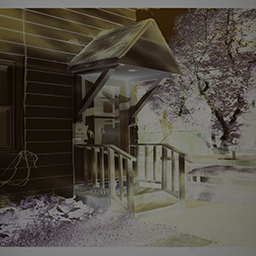
\includegraphics[width=0.4\linewidth]{test.png}
	\caption{The test image}
	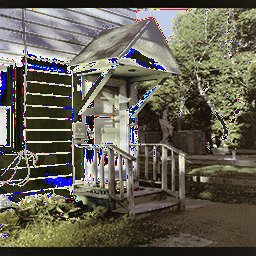
\includegraphics[width=0.4\linewidth]{res.png}
	\caption{Result generated by the current network}
	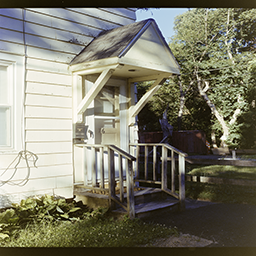
\includegraphics[width=0.4\linewidth]{expected.png}
	\caption{Manual inversion of the same negative}
	\label{fig:test}
\end{figure}
%%%%%%%%%%%%%%%%%%%%%%%%
% Results
%%%%%%%%%%%%%%%%%%%%%%%%
\section{Ablation Study}
\label{sec:ablation}
I have yet to perform an ablation study

%%%%%%%%%%%%%%%%%%%%%%%%%
% Discussion + Conclusion
%%%%%%%%%%%%%%%%%%%%%%%%%
\section{Discussion and Conclusion}
\label{sec:discussion}
So far I'm observing promising results from a preliminary and arguably primitive model, 
but as we can tell there are still noticible artifacts in the generated output.
For the final model, I plan to explore with different models, higher resolution images, 
and a larger and more representative dataset.

%%%%%%%%%%%%%%%%%%%%%%%%%
% References
%%%%%%%%%%%%%%%%%%%%%%%%%
\newpage
\bibliography{references}


\end{document}

